\section{Event Detection Accuracy}
\label{evaluation-sec-eventdetection}

Our network was designed to capture interesting volcanic signals. Thus, it is
critical that the system correctly identify and report such events. This
section evaluates our event detection algorithm both in terms of the number
and rate of event triggers as well as its ability to detect scientifically
interesting events.

\subsection{Event Triggers Per Node}

\begin{figure}[t]
\begin{center}
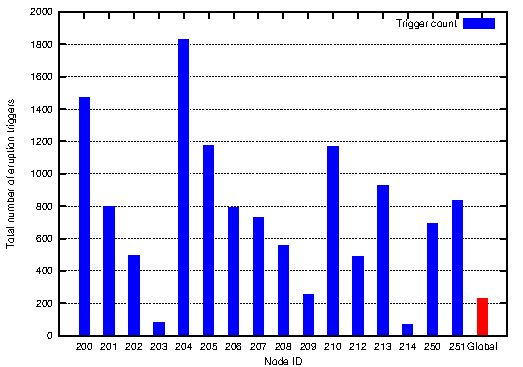
\includegraphics[width=\hsize]{./3-evaluation/figs/eventdetection/eruptionTriggers/eruptCount.pdf}
\end{center}
\caption{\textbf{Event triggers per node.}
This figure shows the total number of event triggers reported by each node.
It demonstrates a wide variation in trigger rates that cannot be attributed
only to varying node uptimes. For example, Node~204 had the lowest uptime but
the largest number of event triggers.}
\label{evaluation-fig-eventspernode}
\end{figure}

\begin{figure}[t]
\begin{center}
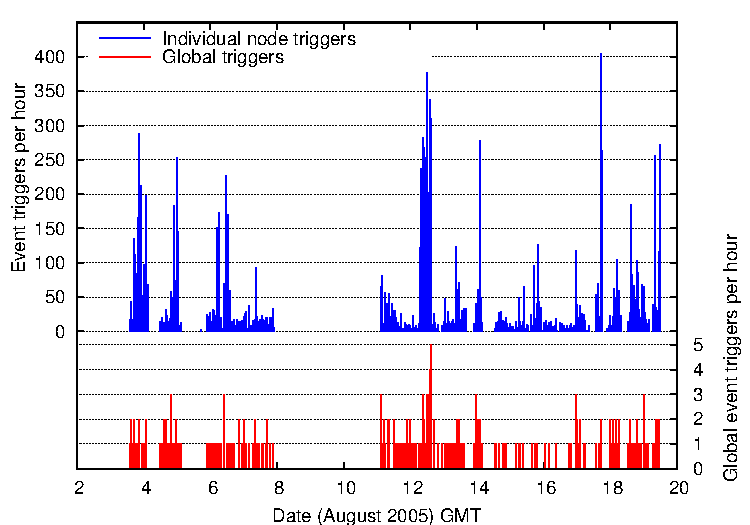
\includegraphics[width=\hsize]{./3-evaluation/figs/eventdetection/eruptionTriggers/eruptCountVsTime.pdf}
\end{center}
\caption{\textbf{Event triggers over time.}
The upper graph shows the total number of individual node triggers per hour.
The lower graph shows the corresponding number of global triggers.
Reventador's varying seismic activity generated between 0~to~5 global
triggers per hour.}
\label{evaluation-fig-eventspertime}
\end{figure}

Figure~\ref{evaluation-fig-eventspernode} shows the total number of events
reported by each node during the deployment. It shows a wide variation in the
event trigger rate, from 70~triggers for Node~213 to 1830~triggers for
Node~204. Variation in the trigger rate can be attributed to many factors,
including the location of the node, the orientation of the seismometer, and
the quality of the seismometer-to-ground coupling. Note that the trigger rate
does not seem to be related to distance from the vent. Although Node~204 was
closest to the vent and reported the most triggers, nodes 200, 205, and 210
all had high trigger counts despite being significantly farther away.

\subsection{Event Triggers Over Time}

Figure~\ref{evaluation-fig-eventspertime} shows both the number of individual
node and global event triggers over each hour. We observe that the volcano's
activity varied greatly, generating trigger counts ranging between~2 and 405
events per hour when the network was online. This activity translates into up
to 5~global event triggers an hour, each initiating a Fetch download cycle of
the associated data.

The volcano's bursty and unpredictable activity makes the network's design
more challenging than systems designed for statically-scheduled data
collection. The data collection protocol, based on our earlier deployment at
Tungurahua~\cite{volcano-ewsn05}, assumed that events would be rare and that
it would be unnecessary to simultaneously record signals for one event while
downloading another. As a result, we missed a number of impressive
back-to-back eruptions typical of the activity at Reventador. It is worth
noting that the variable number of event reports is itself a measure of the
volcano's activity level and could be used to assess hazard levels. 

\subsection{Event Detector Accuracy}
\label{sec-eventdetectaccuracy}

The network detected 229~eruptions, explosions, earthquakes, and tremor
events during the deployment. Ideally, we would like to assess its accuracy
in terms of the fraction of true events detected, as well as the false
positive rate. Given the high degree of coherence required by the global
event detector (requiring 30\% of the active nodes to trigger within a short
time window), we would be surprised if the sensor network recorded any false
events. Indeed, all of the signals we did capture appear to be based on true
volcanic activity, indicating a zero false positive rate.

We intended to apply our event detection algorithm to the signals collected
by the two broadband seismic stations to establish the algorithm's accuracy.
Unfortunately, we found this to be difficult for several reasons. First, each
of the broadband stations suffered intermittent power and software failures,
either preventing them from logging any data, or corrupting the collected
signals or timestamps. Thus, even in those cases where broadband data is
available, it is not always accurate. Second, the broadband stations deployed
a more sensitive seismometer with a much wider frequency response.  The
geophones used by our sensor nodes have a corner frequency of 4.5~Hz, while
the broadband sensors have a corner frequency of 0.033~Hz. Additionally, the
broadband seismometers are much more sensitive, generating voltages of
800~V/m/s, whereas the geophones have a sensitivity of only 32~V/m/s. As a
result, the broadband sensors are able to detect much weaker seismic signals.

We focus our attention on a single day of data where the broadband stations
were recording clean data and the sensor network was relatively stable. One
of our collaborators, a seismologist, visually extracted events from the
broadband data. During this 24-hour period, a total of 589~events were
recorded by the broadband sensors. During the same time, the sensor network
triggered on just 7~events, suggesting that our detection accuracy is very
low: about 1\%.

The network could have failed to detect a seismic event for one of four
reasons: (1) failure of individual nodes; (2) failure of the base station or
radio modem; (3) the low sensitivity of our seismometers; or (4) failure of
the event detection algorithm itself. To factor out the increased sensitivity
of the broadband seismometers, we only consider the 174~events with SNR~$\geq
10$ from both stations, which we expect the geophones should have been able
to detect as well. Also, Section~\ref{evaluation-sec-robustness} has already
addressed the question of uptime, so we focus here on the inherent accuracy
of the event detector when the network was operating correctly. 136~of the
174~broadband events occurred during times when the network was operational.
Taking these two factors into account, the network's detection accuracy is
still only about 5\%. 

Recall that during a Fetch download cycle, nodes disabled sampling to avoid
overwriting data in flash. Download cycles could take up to several minutes
\textit{per node} (see Section~\ref{evaluation-sec-performance}), meaning
that there are significant time windows when the network was unable to detect
new events. During the Fetch cycles on August 15, the broadband stations
recorded 42~events, 24\% of the total events detected. This indicates that,
all else being equal, the sensor network could have detected approximately
24\% more events had we designed the protocol to sample and download
simultaneously. 

In the end, we believe that our low detection rate is the result of the
parameters used in the EWMA-based event detection algorithm. These parameters
were chosen prior to the deployment, based on our experience with detecting
infrasonic events at a different volcano~\cite{volcano-ewsn05}. We did not
experiment with modifying them in the field. Indeed, using our algorithm with
these same parameters on the broadband data for August~15 detects only
101~events, a fraction of the events chosen manually by an expert. 
